\section{Hyper-Heuristics}
\label{sec:hhs}

~\citeauthor{ref:burke:2010}~\cite{ref:burke:2010} define \acp{HH} as search methods or learning mechanism for selecting or generating heuristics to solve computational search problems.~\citeauthor{ref:burke:2003}~\cite{ref:burke:2003} mentions that a \acs{HH} is a high-level approach that, given a particular problem instance and a number of low-level heuristics, can select and apply an appropriate low-level heuristic at each decision point.

\citeauthor{ref:grobler:2015}~\cite{ref:grobler:2015} states that \acp{HH} promote the design of more generally applicable search methodologies and tend to perform relatively well on a large set of different problems, in contrast to specialised algorithms, which typically focus on outperforming the state-of-the-art for a single application.

\acp{HH} implement a form of \index{meta-learning}meta-learning that is concerned with the selection of the best heuristic from a pool of heuristics to solve a given problem. In the context of population-based \acp{HH}, an entity pool exists that represent a pool of candidate solutions to the given problem. Each entity in the entity pool is assigned its own low-level \index{heuristic}heuristic from the heuristic pool.

The selection of the best heuristic to apply to a candidate solution, is based on the performance of the heuristic relative to that particular candidate solution at a particular point in the search process. It can be said that \acp{HH} are concerned with finding the best \index{heuristic}heuristic in \textit{heuristic space}, while the underlying low-level \index{heuristic}heuristics find solutions in the feasible \textit{search/solution space}.

\citeauthor{ref:grobler:2015}~\cite{ref:grobler:2015} highlights two fundamental ideas behind \acp{HH}. Firstly, the recognition that the process of selecting or designing efficient hybrid and/or cooperative heuristics can be regarded as a computational search problem in itself. Secondly, there is significant potential to improve search methodologies by the incorporation of learning mechanisms that can adaptively guide the search. These two fundamental ideas have inspired different types of hyper-heuristics~\cite{ref:burke:2010}.

In the general context of optimisation, many different types of \acp{HH} have been implemented and applied to many different problems. Some notable examples include the \index{simulated annealing}simulated annealing-based \acs{HH} by~\citeauthor{ref:dowsland:2007}~\cite{ref:dowsland:2007}, the \index{tabu-search}tabu-search \acs{HH} of~\citeauthor{ref:burke:2010}~\cite{ref:burke:2010}, the \index{heterogeneous meta-hyper-heuristic}heterogeneous meta-hyper-heuristic by~\citeauthor{ref:grobler:2012}~\cite{ref:grobler:2012} and work done by~\citeauthor{ref:vanderstockt:2018}~\cite{ref:vanderstockt:2018} on the analysis of selection hyper-heuristics for population-based \acp{MH} in real-valued dynamic optimization. Research on the application of \acp{HH} in the context of \acs{FFNN} training is still scarce.~\citeauthor{ref:nel:2021}~\cite{ref:nel:2021} provides the first research in this field, applying a \acs{HH} to \acs{FFNN} training. The following section provides a framework for \acs{HH} classification.

\subsection{Classification of Hyper-Heuristics}\label{sec:hh:classification}

\citeauthor{ref:burke:2010}~\cite{ref:burke:2010} proposed a modern classification scheme used to classify \acp{HH}. According to the proposed classification scheme, \acp{HH} are classified in two dimensions. These include the \textit{source of feedback} used during learning and the nature of the \textit{heuristic search space}. Figure \ref{fig:heuristics:hh:classification} presents the classification scheme as proposed by~\citeauthor{ref:burke:2010}~\cite{ref:burke:2010}.

\begin{figure}[htbp]
	\centering
	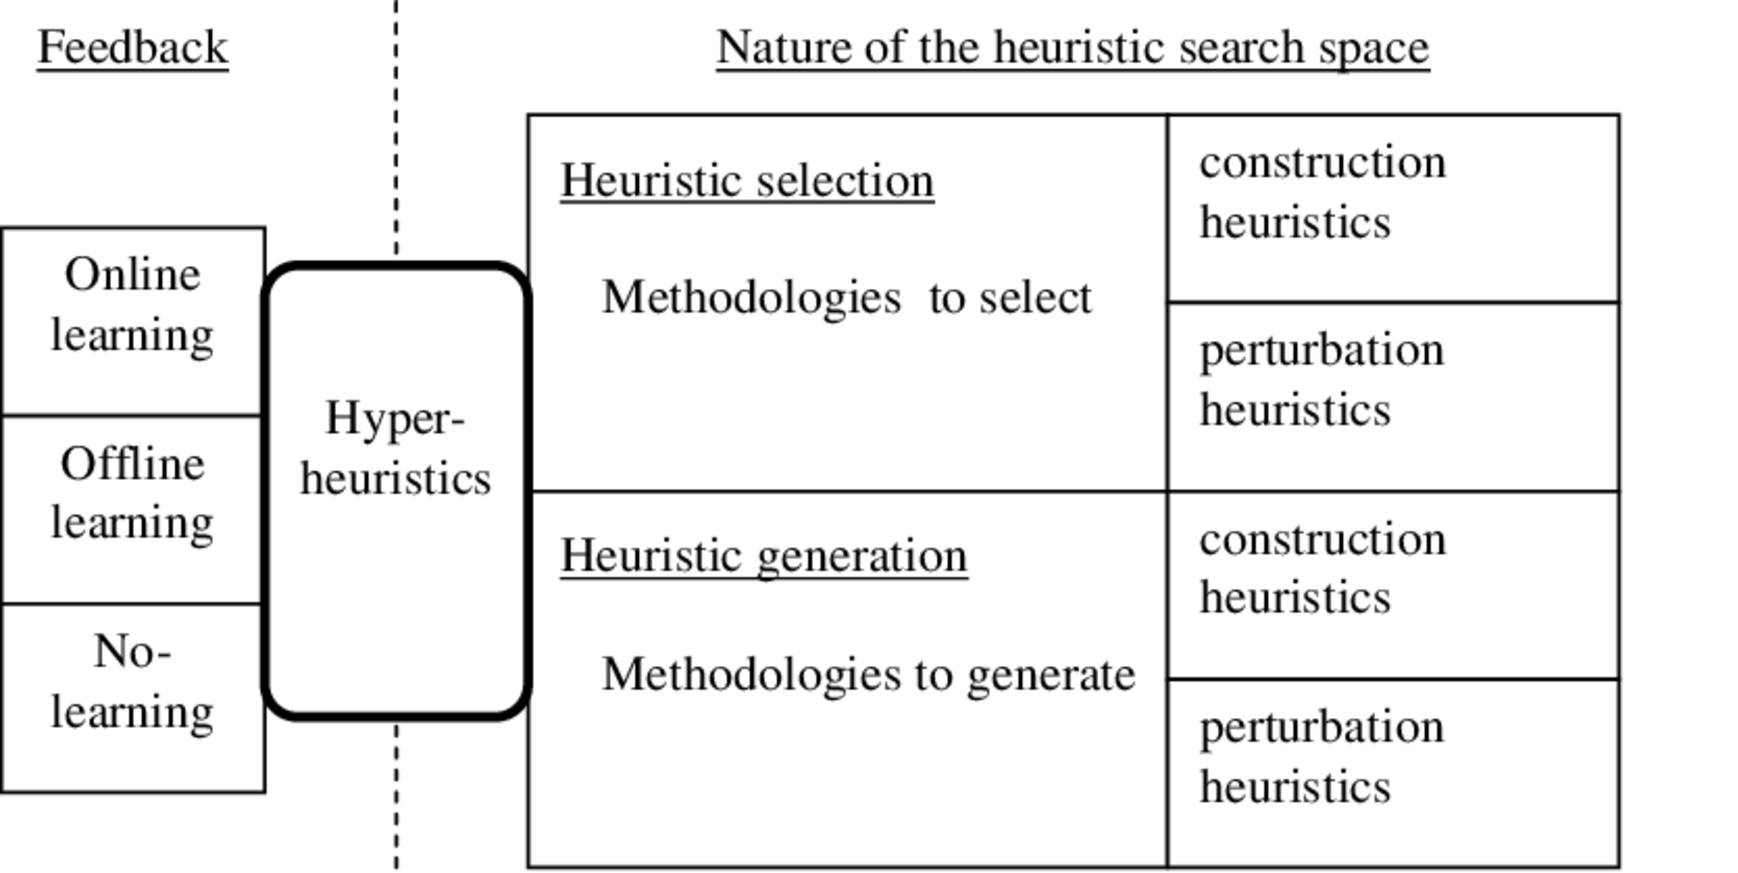
\includegraphics[width=0.85\textwidth]{images/hh_classification.pdf}
	\caption{A classification of \acs{HH} approaches, according to two dimensions: (i) the source of feedback used during learning, and (ii) the nature of the heuristic search space.}
	\label{fig:heuristics:hh:classification}
\end{figure}

\subsubsection{Source of Feedback}

\acp{HH} make use of feedback from the search process to adapt and guide the search process. Some \acp{HH} implement a learning mechanism that utilises this feedback. Learning \acp{HH} can implement a form of \index{online learning}\textit{online learning} or \index{offline learning}\textit{offline learning}.

\acp{HH} that implement \index{online learning}online learning, implement a form of learning that continues to takes place while the algorithm is solving an instance of the underlying optimisation problem. Task-dependent, local properties can be used by the high-level \index{heuristic}heuristic to determine the appropriate low-level heuristic to apply at various points in the search process. Examples of \index{online learning}online learning approaches within \acp{HH} include the use of \acf{RL} and \acfp{MH} as high-level search strategies.

\acp{HH} that implement \index{offline learning}offline learning, implement a form of learning where knowledge, in the form of rules or programs, is gathered from a set of training instances and is then applied independently from the search process itself. Examples of offline learning approaches within hyper-heuristics include \textit{learning classifier systems} and \textit{case-based reasoning}.

\subsubsection{Heuristic Search Space}
According to the classification proposed by~\citeauthor{ref:burke:2010}~\cite{ref:burke:2010}, the second dimension of classification involves the nature of the \index{heuristic}heuristic search space. Distinction is made between \index{heuristic}heuristic \textit{selection} and heuristic \textit{generation}.

\subsubsection{Selection vs. Generation}

Selection \acp{HH} implement a high-level search mechanism that is used to determine which heuristic to apply to the underlying optimisation problem at a given point in the optimisation process. Selection mechanisms can include probabilistic approaches or high level \acfp{MH}. On the contrary, \index{heuristic}heuristic generation methodologies implement a mechanism that generate new heuristics from a pool of \textit{components} of various heuristics. Generation \acp{HH} often make use of \acfp{EA}~\cite{ref:burke:2010}.

Selection \acp{HH} consist of two components, including a low-level \index{heuristic}heuristic selection strategy and a move acceptance strategy. Low-level \index{heuristic}heuristic selection can be done in a simple, \textit{non-adaptive} way. No learning is involved in these approaches. For non-adaptive techniques, heuristic selection is based on a predefined heuristic ordering that is generated either randomly or in a ordered cycle that is repeated throughout the optimisation process~\cite{ref:cowling:2000}. As an alternative, heuristic selection may incorporate an \textit{adaptive} (\index{online learning}\textit{online learning}) mechanism, based on the probabilistic weighting of the low-level heuristics~\cite{ref:burke:2003} or some type of performance statistics~\cite{ref:cowling:2000}.

A move acceptance strategy is the mechanism by which the application of a low-level \index{heuristic}heuristic is either accepted or rejected. In general, a move is accepted or rejected based on the quality of the move and the current solution during a single point search.~\citeauthor{ref:burke:2003}~\cite{ref:burke:2003} mention that many move acceptance strategies have been explored within \acp{HH}.

Move acceptance strategies can be divided into two categories. These include \textit{deterministic} and \textit{non-deterministic} move acceptance strategies. Deterministic move acceptance strategies generate the same result for the same candidate solution(s) used for the move acceptance test. Non-deterministic move acceptance strategies can involve other parameters, such as the current time, or a sampling operation that yields possibly different outcomes when repeated for the move acceptance test~\cite{ref:burke:2003}.


\subsubsection{Construction vs. Perturbation}

Selection and generation \acp{HH} can be further classified in terms of \textit{construction} and \textit{perturbation} mechanisms. According to~\citeauthor{ref:burke:2010}~\cite{ref:burke:2010}, construction approaches build a solution incrementally. Starting with an empty solution, the goal is to intelligently select and use construction heuristics to gradually build a complete solution. As such, the \acs{HH} framework is provided with a set of pre-existing construction heuristics.

Perturbation  approaches refer to approaches that start with a complete solution, generated either randomly or using simple construction heuristics.  Perturbation heuristics try to iteratively improve the current solution. As such, the hyper-heuristic framework is provided with a set of neighbourhood structures and/or simple local searchers.
